%----------------------------------------------------------------------------------------
%	PACKAGES AND OTHER DOCUMENT CONFIGURATIONS
%----------------------------------------------------------------------------------------
\documentclass[12pt]{article}
\usepackage{graphicx}
\usepackage{amsmath,amsfonts,stmaryrd,amssymb} % Math packages
\usepackage{bm}
\usepackage{steinmetz}
\usepackage{enumitem}
\graphicspath{{images/}}
\usepackage{float}
\usepackage{hyperref}
\hypersetup{
	colorlinks=true,
	linkcolor=blue,
	filecolor=magenta,      
	urlcolor=cyan,
	pdftitle={Overleaf Example},
	pdfpagemode=FullScreen,
}
\urlstyle{same}
\usepackage{mathtools}
\usepackage{fancyhdr}
\usepackage{xcolor}
\usepackage[american,RPvoltages]{circuiTikz}
\usepackage{tikz, tikz-cd}
\usepackage{pgfplots}
\usepackage{siunitx}
\usetikzlibrary{spy,shapes,arrows, arrows.meta, bending, decorations.markings}
\pgfplotsset{width=10cm,compat=1.18}
\usepackage{lmodern} % package for changing font size
\usepackage{lastpage}
\renewcommand{\figurename}{Figura}
\usepackage{tcolorbox}
\usepackage{lipsum}
%\usepackage{enumerate} % Custom item numbers for enumerations
\usepackage[ruled]{algorithm2e} % Algorithms
\usepackage[framemethod=tikz]{mdframed} % Allows defining custom boxed/framed environments
\usepackage{listings} % File listings, with syntax highlighting
%\lstset{basicstyle=\ttfamily,} % Typeset listings in monospace font
\usepackage{lipsum}
\tcbuselibrary{listings,theorems,skins,vignette,raster,breakable,magazine,poster,fitting,hooks}
\usepackage[T1]{fontenc}
\usepackage{tgbonum}
 \fontfamily{garamond}
\definecolor{myblue}{RGB}{24, 51, 73}
%----------------------------------------------------------------------------------------
%	DOCUMENT MARGINS
%----------------------------------------------------------------------------------------

\usepackage{geometry} % Required for adjusting page dimensions and margins
\geometry{
	paper=a4paper, % Paper size, change to letterpaper for US letter size
	top=2.5cm, % Top margin
	bottom=3cm, % Bottom margin
	left=2cm, % Left margin
	right=2.5cm, % Right margin
	headheight=14pt, % Header height
	footskip=1.5cm, % Space from the bottom margin to the baseline of the footer
	headsep=1.2cm, % Space from the top margin to the baseline of the header
	%showframe, % Uncomment to show how the type block is set on the page
}

%----------------------------------------------------------------------------------------
%	FONTS
%----------------------------------------------------------------------------------------

\usepackage[utf8]{inputenc} % Required for inputting international characters
\usepackage[T1]{fontenc} % Output font encoding for international characters
\usepackage{XCharter} % Use the XCharter fonts
\usepackage{tgbonum}

\makeatletter
\pgfcircdeclarebipole{}{\ctikzvalof{bipoles/vsourcesin/height}}{sVpm}{\ctikzvalof{bipoles/vsourcesin/height}}{\ctikzvalof{bipoles/vsourcesin/width}}{
	
	\pgfsetlinewidth{\pgfkeysvalueof{/tikz/circuitikz/bipoles/thickness}\pgfstartlinewidth}
	\pgfpathellipse{\pgfpointorigin}{\pgfpoint{0}{\pgf@circ@res@up}}{\pgfpoint{\pgf@circ@res@left}{0}}
	\pgfusepath{draw}     
	\pgftext[bottom,rotate=90,y=\ctikzvalof{bipoles/vsourceam/margin}\pgf@circ@res@down]{\scriptsize$-$}
	\pgftext[top,rotate=90,y=\ctikzvalof{bipoles/vsourceam/margin}\pgf@circ@res@up]{\scriptsize$+$}
	
	\pgf@circ@res@up = .35\pgf@circ@res@up
	\pgfscope
	\pgftransformrotate{90}
	\pgfpathmoveto{\pgfpoint{-\pgf@circ@res@up}{0cm}}
	\pgfpathsine{\pgfpoint{.5\pgf@circ@res@up}{.4\pgf@circ@res@up}}
	\pgfpathcosine{\pgfpoint{.5\pgf@circ@res@up}{-.4\pgf@circ@res@up}}
	\pgfpathsine{\pgfpoint{.5\pgf@circ@res@up}{-.4\pgf@circ@res@up}}
	\pgfpathcosine{\pgfpoint{.5\pgf@circ@res@up}{.4\pgf@circ@res@up}}
	\pgfusepath{draw}
	\endpgfscope
}
\def\pgf@circ@sVpm@path#1{\pgf@circ@bipole@path{sVpm}{#1}}
\compattikzset{sinusoidal voltage source pm/.style = {\circuitikzbasekey, /tikz/to path=\pgf@circ@sVpm@path, \circuitikzbasekey/bipole/is voltage=true, \circuitikzbasekey/bipole/is voltageoutsideofsymbol=true, v=#1 }}
\compattikzset{sVpm/.style = {\comnpatname sinusoidal voltage source pm = #1}}

\pgfcircdeclarebipole{}{\ctikzvalof{bipoles/vsourcesin/height}}{sVpmh}{\ctikzvalof{bipoles/vsourcesin/height}}{\ctikzvalof{bipoles/vsourcesin/width}}{
	
	\pgfsetlinewidth{\pgfkeysvalueof{/tikz/circuitikz/bipoles/thickness}\pgfstartlinewidth}
	\pgfpathellipse{\pgfpointorigin}{\pgfpoint{0}{\pgf@circ@res@up}}{\pgfpoint{\pgf@circ@res@left}{0}}
	\pgfusepath{draw}     
	\pgftext[center,x=0.2\pgf@circ@res@down-\ctikzvalof{bipoles/vsourceam/margin}\pgf@circ@res@down]{\scriptsize$-$}
	\pgftext[top,rotate=90,y=\ctikzvalof{bipoles/vsourceam/margin}\pgf@circ@res@up]{\scriptsize$+$}
	
	\pgf@circ@res@up = .35\pgf@circ@res@up
	\pgfscope
	\pgftransformrotate{90}
	\pgfpathmoveto{\pgfpoint{-\pgf@circ@res@up}{0cm}}
	\pgfpathsine{\pgfpoint{.5\pgf@circ@res@up}{.4\pgf@circ@res@up}}
	\pgfpathcosine{\pgfpoint{.5\pgf@circ@res@up}{-.4\pgf@circ@res@up}}
	\pgfpathsine{\pgfpoint{.5\pgf@circ@res@up}{-.4\pgf@circ@res@up}}
	\pgfpathcosine{\pgfpoint{.5\pgf@circ@res@up}{.4\pgf@circ@res@up}}
	\pgfusepath{draw}
	\endpgfscope
}
\def\pgf@circ@sVpmh@path#1{\pgf@circ@bipole@path{sVpmh}{#1}}
\compattikzset{sinusoidal voltage source pmh/.style = {\circuitikzbasekey, /tikz/to path=\pgf@circ@sVpmh@path, \circuitikzbasekey/bipole/is voltage=true, \circuitikzbasekey/bipole/is voltageoutsideofsymbol=true, v=#1 }}
\compattikzset{sVpmh/.style = {\comnpatname sinusoidal voltage source pmh = #1}}
\makeatother


%----------------------------------------------------------------------------------------
%	BEGIN DOCUMENT
%----------------------------------------------------------------------------------------

\begin{document}
	%\thispagestyle{empty}
	\begin{tikzpicture}[remember picture, overlay]
		\node[anchor=north west, inner sep=0pt] at (current page.north west) {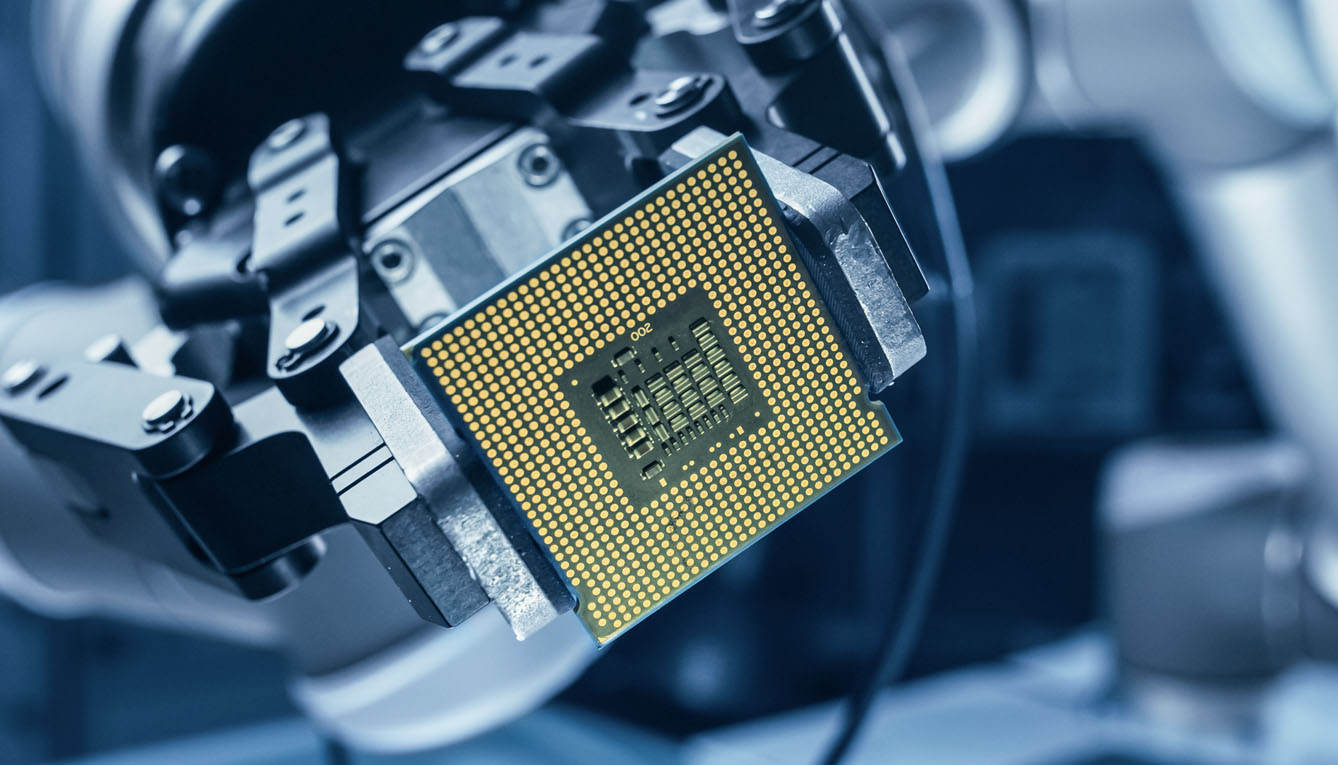
\includegraphics[width=\paperwidth, height=.5\paperheight]{picture1}};
	\end{tikzpicture}

	\vspace{13cm}
	\noindent \textcolor{myblue}{\fontsize{40pt}{40pt}\selectfont \textbf{The SPICE Diode Model}}\\\\\\
	{\fontsize{18pt}{18pt}\selectfont Special Acknowledgment\\\\}
	This chapter was written by Howard T. Russel, Jr., PhD, OPAL Engineering, Inc., August 4, 1991, under contract with Motorola Inc. Opal Engineeting is located at 828 Opal Drive, Suite 1, San Jose, CA 95117. 
	
	\newpage
	\section*{Introduction}
	This chapters presents a description of the SPICE diode model and methods for the extraction of its parameters. A comprehensive examination of this model will be given along with comparisons of the characteristics of a real diodo and those produced by the model. These comparisons will be used to illustrate the model's accuracy and limitations. Based on the nature of the model equations, mathematical methods for the extraction of the SPICE parameters (with the exception of the noise parameters) will be presented. These methods are easily implemented for a motorola MURH840CT rectifiar as example. Throughout this chapter, references are made to the characteristics and bhavior of an ideal diode model. The development of this model may be found in severalof the many wll-known texts on the subjects of semiconductor device theory and $pn$ juntion diodes.\\
	
	The SPICE model of a $pn$ junction diode consists of mathematical equations, parameters, and variables, all of which are designed to work together to simulate as accurately as possible the electrical characteristics of a real device. The equations and variables used for the model in the SPICE program are fixed and not easily modified. Therefore, the accuracy resulting from a SPICE simulation of a diode depends on the precise extraction methods which can be applied to this model, some of which yield more accurace results than others. The inherent success of a particular method depends for the most part on how well device physics and theory are utilized in the design of the model, and upon the availability of data taken from a real device. 
	
	\section*{The SPICE Diode Model}
	The parameters for the SPICE model of the diode are given in Table 3.1. The equations that use these parameters are divided into four model groups which are responsible for simulation various diode characteristics. These groups consists of the large-signal dc model, the small signal ac model, temperature and area effects, and the noise model.
	
	\subsection*{The Large-signal DC Model}
	The large-signal behavior of the SPICE diode is characterized by the relationship between the dc current and voltage at its terminals. The parameters used to model this behavior are IS, RS, N, BV y IBV. The parameters IS is the same as the reverse saturation current $I_s$ for an ideal diode. The ohmic resistance RS is sued to model the resistance of the metal contacts and the neutral regions under high-level injection. The emission coefficient N is used to modify the slope of the current versus voltage (I-V) characteristic curve. Finally, the parameters BV and IBV model the reverse breakdown behavior.
	Figure 3.1 shows the equivalent circuits of the SPICE diode for large-signal dc analysis. This circuit contains an internal diode $D_1$, a series resistance having a value of RS, and a shunt conductance GMIN. The SPICE program adds this conductance, which is transparent to the user, around every internal $pn$ junction to aid convergence. The program default value for GMIN is $10^{-12}$ mhos but can be set to any other nonzero value with a .OPTIONS line in the circuit file.
	
	\begin{figure}[H]
		\centering	
		\begin{tikzpicture}[scale=0.8]
			\draw (0,0) coordinate(p0) node[left]{$-$} to[short, o-*] ++(4,0)
						to[D*, invert, -*, v>=$V_D$, l=$D_1$] ++(0,4) coordinate(n1)
						to[R, l_=$RS$] ++(0,4)
						to[short, -o, f<_=$I_D$]  ++(-4,0) coordinate(p1) node[left]{$+$};
			\draw (n1)  to[short] ++(4,0)
						to[R, l=$G_{min}$] ++(0,-4)
						to[short] ++(-4,0);
			\coordinate (M) at ($(p0)!0.5!(p1)$);
			\draw (M) node[]{$V_F$} coordinate(in);
			\draw  [->] ($(in)+(0,0.4)$) -- ($(p1)+(0,-0.2)$) ;
			\draw  [->] ($(in)+(0,-0.4)$) -- ($(p0)+(0,+0.2)$) ;
			\draw[dashed] ($(p1)+(2.6,1)$) rectangle ($(p0)+(10,-1)$);
		\end{tikzpicture}
		\caption{Amplificador multietapa}	
		\label{fig:figura1}
	\end{figure}
	
	The dc model variables consists of the voltage across the external diode terminals $V_F$, the voltage  across the interbal diode terminals $V_D$, and terminal current $I_D$. With this parameters and variables, the large-signal dc characteristics are modeled by the following equations. 
	
	\begin{align}
		V_F = RS \cdot I_D + V_D
	\end{align}

	\noindent y
	
	\begin{align}
		I_D = f(V_D)
	\end{align}
	
	\noindent Where four regions of operation describe the functional relationship between the internal diode voltage and the diode current.
	
	\begin{tcolorbox}[colback=red!5!white,colframe=red!75!black,arc=0mm,boxrule=0mm,width=(\linewidth+0.5cm)]
		\begin{equation}
			I_{C1} = \frac{\beta}{\beta + 1}I_{ref}
		\end{equation}
	\end{tcolorbox}
	
	\noindent Donde
	\begin{tcolorbox}[colback=red!5!white,colframe=red!75!black,arc=0mm,boxrule=0mm,width=(\linewidth+0.5cm)]
		\begin{equation}
			I_{ref} = \frac{V_{CC} - V_{BE}}{R_1}
		\end{equation}
	\end{tcolorbox}
	
	\noindent Para $\beta \gg 1$
	\begin{align}
		I_{ref} \cong I_{C1}
	\end{align}
	
	\subsection*{Ejemplo}
	Disele una fuente de corriente Widlar para generar una corriente constante $I_o = \SI{10}{\micro\ampere}$. Asuma que $V_{CC} = \SI{10}{\volt}, V_{BE} = \SI{0.7}{\volt}, \beta=125$. Use $V_T = \SI{25}{\milli\volt}$.
	
	
	\noindent Para la fuente de corriente Widlar primero debemos decidir un valor apropiado para $I_ref$. Si escogemos $I_{ref} = \SI{1}{\milli\ampere}$, entonces $R_1$ está dado por
	\begin{align}
		R_1 = \frac{\SI{10}{\volt} - \SI{0.7}{\volt}}{\SI{1}{\milli\ampere}} = \SI{9.3}{\kilo\ohm}
	\end{align}
	
	\noindent El valor de $R_E$ está dado por la ecuación (7)
	\begin{align}
		R_E = \frac{\SI{25}{\milli\volt}}{\left(1 + \frac{1}{125}\right)\SI{10}{\micro\ampere}}\ln \left( \frac{\SI{1}{\milli\ampere}}{\SI{10}{\micro\ampere}} \right) = \SI{11.5}{\kilo\ohm}
	\end{align}
	
	\noindent Es claro ver que el circuito de Widlar permite la generación de constantes pequeñas usando resistores relativamente pequeños.
\end{document}